\documentclass[12pt]{article}

\usepackage{sbc-template}
\usepackage{graphicx,url}
\usepackage[utf8]{inputenc}
\usepackage[brazil]{babel}
\usepackage{multirow}
\usepackage{amsmath}
\usepackage{xcolor}
\usepackage{pbox}
\usepackage{tikz}

\newcommand{\lembrete}[1]{{\color{blue}{#1}}}

\newcommand{\aspas}[1]{``{#1}''}
     
\sloppy

\title{Relatório da implementação do Robo}

\author{Gustavo José Neves da Silva\inst{1}\\Wilton Jaciel Loch\inst{1}}

\address{Departamento de Ciência da Computação\\
  Universidade do Estado de Santa Catarina (UDESC) -- Joinville, SC -- Brasil
  \email{gustavo.neves@yandex.com, wilton.loch@hotmail.com.br}
}	
				

\begin{document} 

\maketitle

%\begin{abstract}
%  abstract
%\end{abstract}
     
\begin{resumo}
%  Este meta-artigo descreve o estilo a ser usado na confecção de artigos e
%  resumos de artigos para publicação nos anais das conferências organizadas
%  pela SBC. É solicitada a escrita de resumo e abstract apenas para os artigos
%  escritos em português. Artigos em inglês deverão apresentar apenas abstract.
%  Nos dois casos, o autor deve tomar cuidado para que o resumo (e o abstract)
%  não ultrapassem 10 linhas cada, sendo que ambos devem estar na primeira
%  página do artigo.
O presente trabalho realizado como parte da disciplina de Inteligência Artificial propõe uma implementação de um sistema de navegação automática de um robô responsável por diferentes manutenções em unidades fabris, utilizando o algoritmo $A^{*}$ para calcular o custo da rota, exibindo o custo do caminho percorrido pelo robô enquanto ele se movimenta pelo mapa e também o custo final ao terminar a execução.
\end{resumo}

\section{Introdução} \label{sec:Introducao}
Esse trabalho propõe uma implementação de um sistema de navegação automática de um robô responsável por diferentes manutenções em unidades fabris.
%
As únicas informações que o robô possui são a informações da posição das fábricas, quantas e quais ferramentas cada uma delas necessita.
%
As ferramentas estão espalhadas no ambiente e o robô não possui informação quanto a sua localização.

\textbf{Tipos de ferramentas existentes no sistema:}
\begin{itemize}
	\item Bateria de carga elétrica
	\item Braço de solda;
	\item Bomba de sucção;
	\item Dispositivo de refrigeração;
	\item Braço pneumático;
\end{itemize}

\textbf{Características do robô:}
\begin{itemize}
	\item Possui um alcance máximo de 4 regiões adjacentes em todas as direções com o qual analisa o ambiente a fim de obter as informações do terreno e do que está sobre ele
	\item Somente se desloca na vertical e na horizontal
	\item A posição inicial é configurável por um arquivo de entrada
	\item Representado no ambiente por: \tikz\draw[black,fill=white] (0,0) rectangle (0.35,0.35);
\end{itemize}
%
%O robô possui um alcance máximo de 4 regiões adjacentes em todas as direções com o qual analisa o ambiente a fim de obter as informações do terreno e do que está sobre ele.
%
%O robô somente se desloca na vertical e na horizontal
%
%O ambiente é configurável por arquivo de entrada
%
%A posição inicial do robô e das fábricas são configuráveis por um arquivo de entrada
%
%As ferramentas apesar de serem dispostas de forma aleatória, estão sempre localizadas em terrenos de custo 1. 
%
%O programa exibe o custo do caminho percorrido pelo agente enquanto ele se movimenta pelo mapa e também o custo final ao terminar a execução
%
%Obstáculos podem ser inseridos ou removidos durante a configuração do ambiente.

\textbf{Total de cada tipo de ferramenta e suas cores de representação no ambiente:}
\begin{itemize}
	\item 20 baterias de carga elétrica - \tikz\draw[red,fill=red] (0,0) circle (.5ex); 
	\item 10 braços de solda - \tikz\draw[yellow,fill=yellow] (0,0) circle (.5ex);
	\item 8 bombas de sucção - \tikz\draw[magenta,fill=magenta] (0,0) circle (.5ex);
	\item 6 dispositivos de refrigeração - \tikz\draw[cyan,fill=cyan] (0,0) circle (.5ex);
	\item 4 braços pneumáticos - \tikz\draw[blue,fill=blue] (0,0) circle (.5ex);
\end{itemize}

\textbf{Tipos de fábricas, suas necessidades e suas cores de representação no ambiente:}
\begin{itemize}
	\item Indústria de melhoramento genético de grãos, necessita de 8 baterias de carga elétrica - \tikz\draw[red,fill=red] (0,0) rectangle (0.35,0.35);
	\item Empresa de manutenção de cascos de embarcações, necessita de 5 braços de solda - \tikz\draw[yellow,fill=yellow] (0,0) rectangle (0.35,0.35);
	\item Indústria petrolífera com dutos entupidos, necessita de 2 bombas de sucção - \tikz\draw[magenta,fill=magenta] (0,0) rectangle (0.35,0.35);
	\item Fábrica de fundição, necessita de 5 dispositivos de refrigeração - \tikz\draw[cyan,fill=cyan] (0,0) rectangle (0.35,0.35);
	\item Indústria de vigas de aço, necessita de 2 braços pneumáticos - \tikz\draw[blue,fill=blue] (0,0) rectangle (0.35,0.35);
\end{itemize}

%O trabalho consiste em implementar um sistema de navegação automática de um robô que realiza
%diferentes manutenções em unidades fabris. Para isto, deve-se utilizar o algoritmo de busca A* para
%o cálculo do custo da rota.
%
%O robô tem a informação da posição das fábricas a serem realizadas as manutenções, mas está
%desprovido de ferramentas para realizá-las. As ferramentas estão dispersas no ambiente e o robô
%deve capturá-las utilizando seu radar para poder se dirigir para a fábrica. Ou seja, o agente não tem
%a informação da localidade das ferramentas e só pode realizar a manutenção se possuir a ferramenta
%necessária.
%Existem 5 tipos de ferramentas dispersas no ambiente:
%• Bateria de carga elétrica;
%• Braço de solda;
%• Bomba de sucção;
%• Dispositivo de refrigeração;
%• Braço pneumático.
%A posição inicial das ferramentas é desconhecida. O agente deve utilizar seu radar para localizá-las.
%O radar possui um alcance máximo de 4 regiões adjacentes em todas as direções. 

\section{Metodologia de Desenvolvimento} \label{sec:Desenvolv}
A linguagem utilizada na implementação foi C++, por sua robustez, variedade de ferramentas e desempenho. Para representação gráfica dos componentes(robô, ferramentas e fabricas) foi utilizada a biblioteca SFML, que oferece uma plataforma simplificada para o uso de gráficos em duas dimensões. O ambiente é representado por uma matriz 42 x 42 e é configurável por arquivo de entrada.
%
Tal que:

\textbf{Os tipos de terrenos que compõem o ambiente, suas respectivos custos e cores:}
\begin{itemize}
	\item Sólido e plano – Custo: 1 - \tikz\draw[black,fill={rgb,255:red,146; green,208; blue,80}] (0,0) rectangle (0.35,0.35);
	\item Montanhoso – Custo: 5 - \tikz\draw[black,fill={rgb,255:red,148; green,138; blue,84}] (0,0) rectangle (0.35,0.35);
	\item Pântano – Custo: 10 - \tikz\draw[black,fill={rgb,255:red,84; green,141; blue,212}] (0,0) rectangle (0.35,0.35);
	\item Árido – Custo: 15 - \tikz\draw[black,fill={rgb,255:red,227; green,108; blue,10}] (0,0) rectangle (0.35,0.35);
	\item Obstáculo – Intransponível - \tikz\draw[black,fill=black] (0,0) rectangle (0.35,0.35);
\end{itemize}

\begin{figure}[ht]
\centering
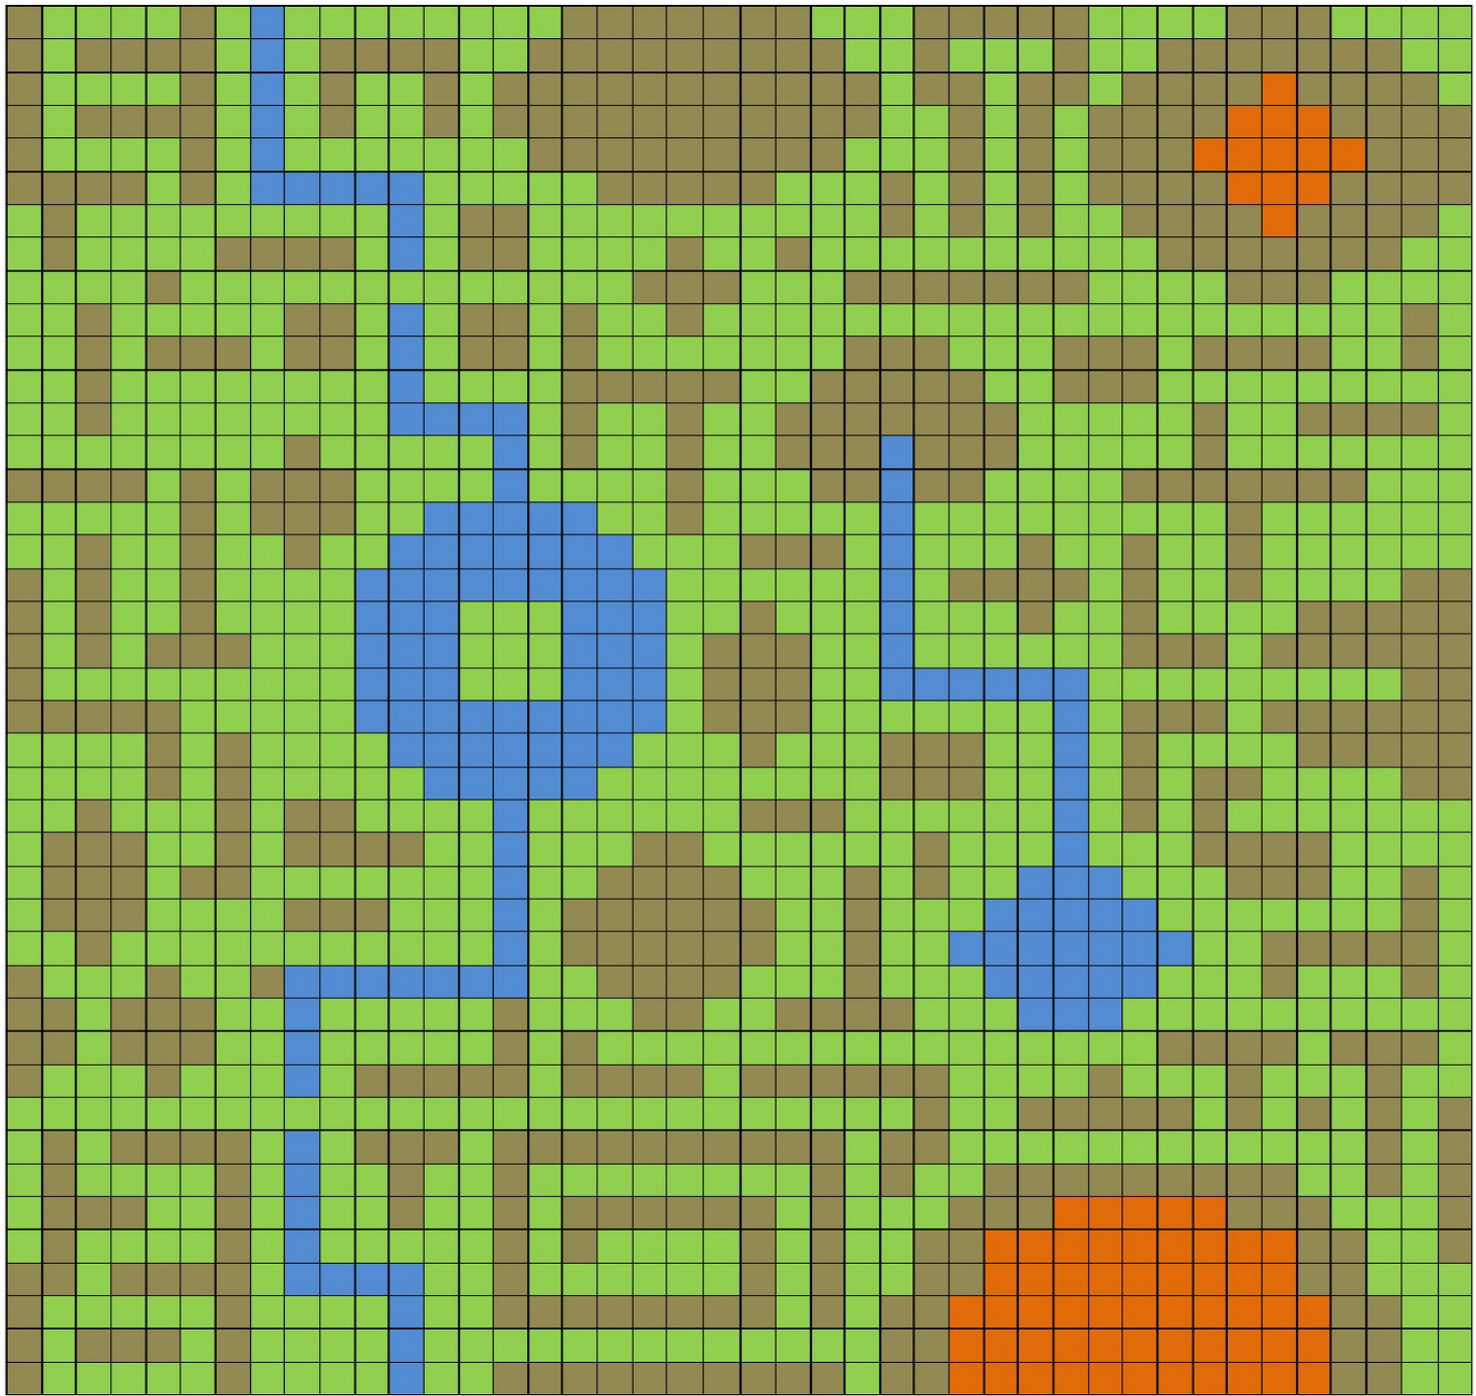
\includegraphics[width=.5\textwidth]{imagens/terreno}
\caption{Ambiente explorado pelo robô}
\label{fig:ambiente}
\end{figure}

%	Tem a classe robô, lá que acontece tudo.
%A função seguir caminho
%	 é a que faz ele propriamente caminhar
%	 e é lá também que são chamados outros funções pra verificar se na nova posição dele(a que ele acabou de se mexer) é possível pegar uma ferramenta ou atender uma fábrica. 
%	 
%	 Dentro de seguir caminho também é que é chamado a função escolherDestino que é como se fosse o cérebro do robô pra tomar as decisões sobre pra onde ir. 
%	 
%	 
\textbf{O algoritmo de decisão do robô funciona da seguinte forma:}
\begin{itemize}
	\item Se não há ferramentas escaneadas e ainda nenhuma fábrica pode ser atendida, vá para a fábrica mais próxima
	\item Se uma ferramenta for escaneada e ainda não há ferramentas suficientes daquele tipo, vá até a ferramenta e pegue-a
	\item Se estiver muito próximo (2 unidades de distância) de uma fábrica que ainda não pode ser atendida e não houver ferramentas escaneadas, vá para a fábrica mais distante
	\item Se muito próximo do destino do passo anterior(fábrica mais distante) e não houver ferramentas escaneadas, vá para um ponto de interesse(pontos próximos da borda do mapa em posições distintas)
\end{itemize}

O caminho do robô é representado por uma pilha de direções (0 a 3 no sentido horário) que são desempilhadas uma a uma para que o robô possa realizar um movimento. 
Toda vez que é definido que o robô deve ir para uma fábrica, ferramenta ou qualquer outro destino ele executa o $A^{*}$ da posição atual até o ponto desejado. 
As ferramentas encontradas são subtraídas da quantidade faltando até que chegue em zero. 

%	 O cérebro do robô em si funciona assim: 
%	 	Se não há ferramentas escaneadas e ainda nenhuma fábrica pode ser atendida, vá para a fábrica mais próxima. 		
%	 	Se uma ferramenta for escaneada e ainda não há ferramentas suficientes daquele tipo, vá até a ferramenta e pegue-a. 
%	 	Se estiver muito próximo (2 de distância) de uma fábrica que ainda não pode ser atendida e não houver ferramentas escaneadas, vá para a fábrica mais distante. 
%	 	Se muito próximo do destino do passo anterior(fábrica mais distante) e não houver ferramentas escaneadas, vá para um ponto de interesse.
%	 	Pontos de interesse são basicamente pontos próximos da borda do mapa em posições distintas.
\section{Descrição de Experimentos/Simulações e Resultados Obtidos} \label{sec:DescExp}
Realizadas 20 execuções consecutivas, cujos resultados foram armazenados em arquivos para posterior análise a fim de se obter o comportamento médio do sistema.

\section{Análise dos resultados obtidos} \label{sec:Results}
\begin{table}[h]
	\centering
	\begin{tabular}{|l|c|}
	\hline
	& Custo total \\ \hline
	Min. & 322.0 \\ \hline
	$1^{o}$ quartil & 393.8 \\ \hline
	Mediana & 458.0 \\ \hline
	Media & 475.4 \\ \hline
	$3^{o}$ quartil & 531.5 \\ \hline
	Máx. & 750.0 \\ \hline
	\end{tabular}
	\caption{Análise custo total}
	\label{tabela:custo}
%%	
%%"" "Min.   :322.0  "
%%"" "1st Qu.:393.8  "
%%"" "Median :458.0  "
%%"" "Mean   :475.4  "
%%"" "3rd Qu.:531.5  "
%%"" "Max.   :750.0  "
%%
\end{table}

\begin{table}[h]
	\centering
	\begin{tabular}{|l|c|}
	\hline
	& Destinos escolhidos \\ \hline
	Min. & 27.00 \\ \hline
	$1^{o}$ quartil & 28.75 \\ \hline
	Mediana & 30.00 \\ \hline
	Media & 30.65 \\ \hline
	$3^{o}$ quartil & 32.25 \\ \hline
	Máx. & 37.00 \\ \hline
	\end{tabular}
	\caption{Análise destinos escolhidos}
	\label{tabela:destinos}
%%	
%%"      V1"
%%"" "Min.   :27.00  "
%%"" "1st Qu.:28.75  "
%%"" "Median :30.00  "
%%"" "Mean   :30.65  "
%%"" "3rd Qu.:32.25  "
%%"" "Max.   :37.00  "
%%
\end{table}


\begin{table}[h]
	\centering
	\begin{tabular}{|l|c|}
	\hline
	& Num. movimentos realizados \\ \hline
	Min. & 297.0 \\ \hline
	$1^{o}$ quartil & 340.5 \\ \hline
	Mediana & 410.0 \\ \hline
	Media & 419.9 \\ \hline
	$3^{o}$ quartil & 459.0 \\ \hline
	Máx. & 651.0 \\ \hline
	\end{tabular}
	\caption{Análise movimentos realizados}
	\label{tabela:movimentos}
%%
%%"      V1"
%%"" "Min.   :297.0  "
%%"" "1st Qu.:340.5  "
%%"" "Median :410.0  "
%%"" "Mean   :419.9  "
%%"" "3rd Qu.:459.0  "
%%"" "Max.   :651.0  "
%%
\end{table}


\begin{table}[h]
	\centering
	\begin{tabular}{|l|c|}
	\hline
	& Num. nós expandidos \\ \hline
	Min. & 6219 \\ \hline
	$1^{o}$ quartil & 8916 \\ \hline
	Mediana & 11220 \\ \hline
	Media & 12006 \\ \hline
	$3^{o}$ quartil & 14764 \\ \hline
	Máx. & 21126 \\ \hline
	\end{tabular}
	\caption{Análise nós expandidos}
	\label{tabela:nosExpandidos}
%%	
%%"      V1"
%%"" "Min.   : 6219  "
%%"" "1st Qu.: 8916  "
%%"" "Median :11220  "
%%"" "Mean   :12006  "
%%"" "3rd Qu.:14764  "
%%"" "Max.   :21126  "
%%
\end{table}
\section{Conclusões e Trabalhos Futuros} \label{sec:Conclusoes}
Como observado nas tabelas \ref{tabela:custo} e \ref{tabela:nosExpandidos}, o valor do custo em média é baixo(475.4), porém o número de nós expandidos ainda é elevado(12006). Como trabalhos futuros é pretentido otimizar abordagem utilizada visando reduzir o número de nós expandidos e analisar se há alguma correlação entre esse valor e os demais analisados no sistema(custo total, número de movimentos realizados, número de destinos escolhidos)
\bibliographystyle{sbc}
\bibliography{arqReferencias}

\end{document}

%
%\section{Figures and Captions}\label{sec:figs}
%
%
%Figure and table captions should be centered if less than one line
%(Figure~\ref{fig:exampleFig1}), otherwise justified and indented by 0.8cm on
%both margins, as shown in Figure~\ref{fig:exampleFig2}. The caption font must
%be Helvetica, 10 point, boldface, with 6 points of space before and after each
%caption.
%
%\begin{figure}[ht]
%\centering
%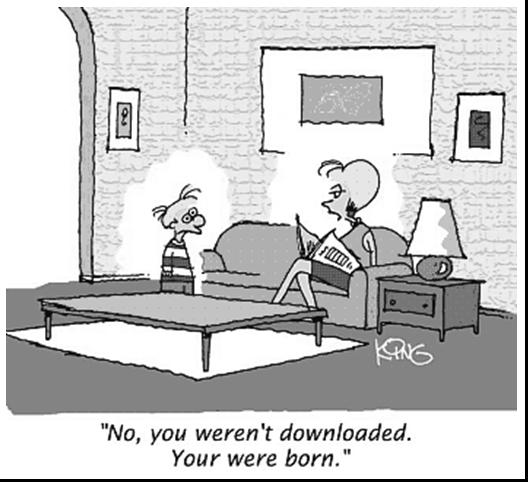
\includegraphics[width=.5\textwidth]{fig1.jpg}
%\caption{A typical figure}
%\label{fig:exampleFig1}
%\end{figure}
%
%\begin{figure}[ht]
%\centering
%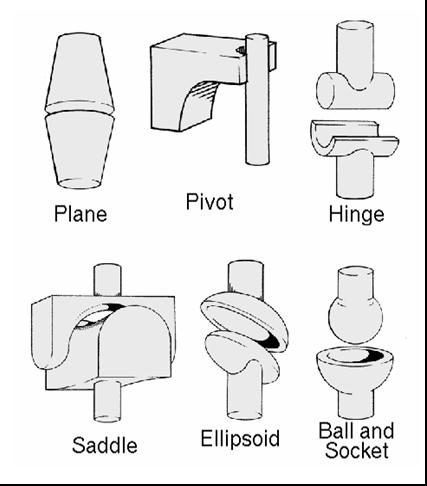
\includegraphics[width=.3\textwidth]{fig2.jpg}
%\caption{This figure is an example of a figure caption taking more than one
%  line and justified considering margins mentioned in Section~\ref{sec:figs}.}
%\label{fig:exampleFig2}
%\end{figure}
%
%In tables, try to avoid the use of colored or shaded backgrounds, and avoid
%thick, doubled, or unnecessary framing lines. When reporting empirical data,
%do not use more decimal digits than warranted by their precision and
%reproducibility. Table caption must be placed before the table (see Table 1)
%and the font used must also be Helvetica, 10 point, boldface, with 6 points of
%space before and after each caption.
%
%\begin{table}[ht]
%\centering
%\caption{Variables to be considered on the evaluation of interaction
%  techniques}
%\label{tab:exTable1}
%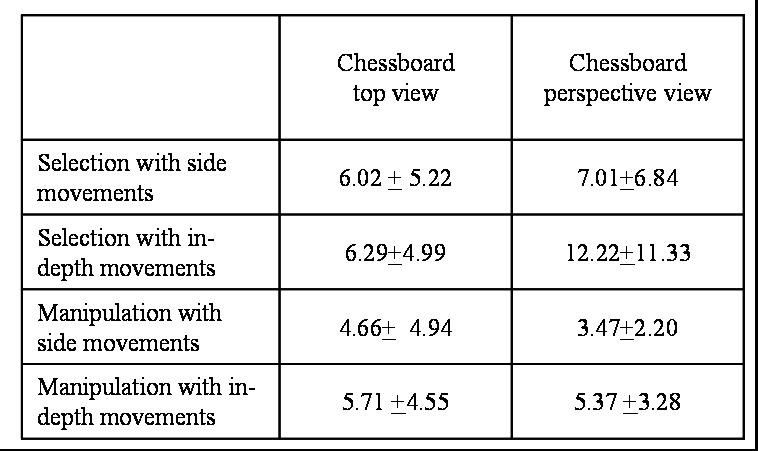
\includegraphics[width=.7\textwidth]{table.jpg}
%\end{table}
%
